\begin{figure}[t!]
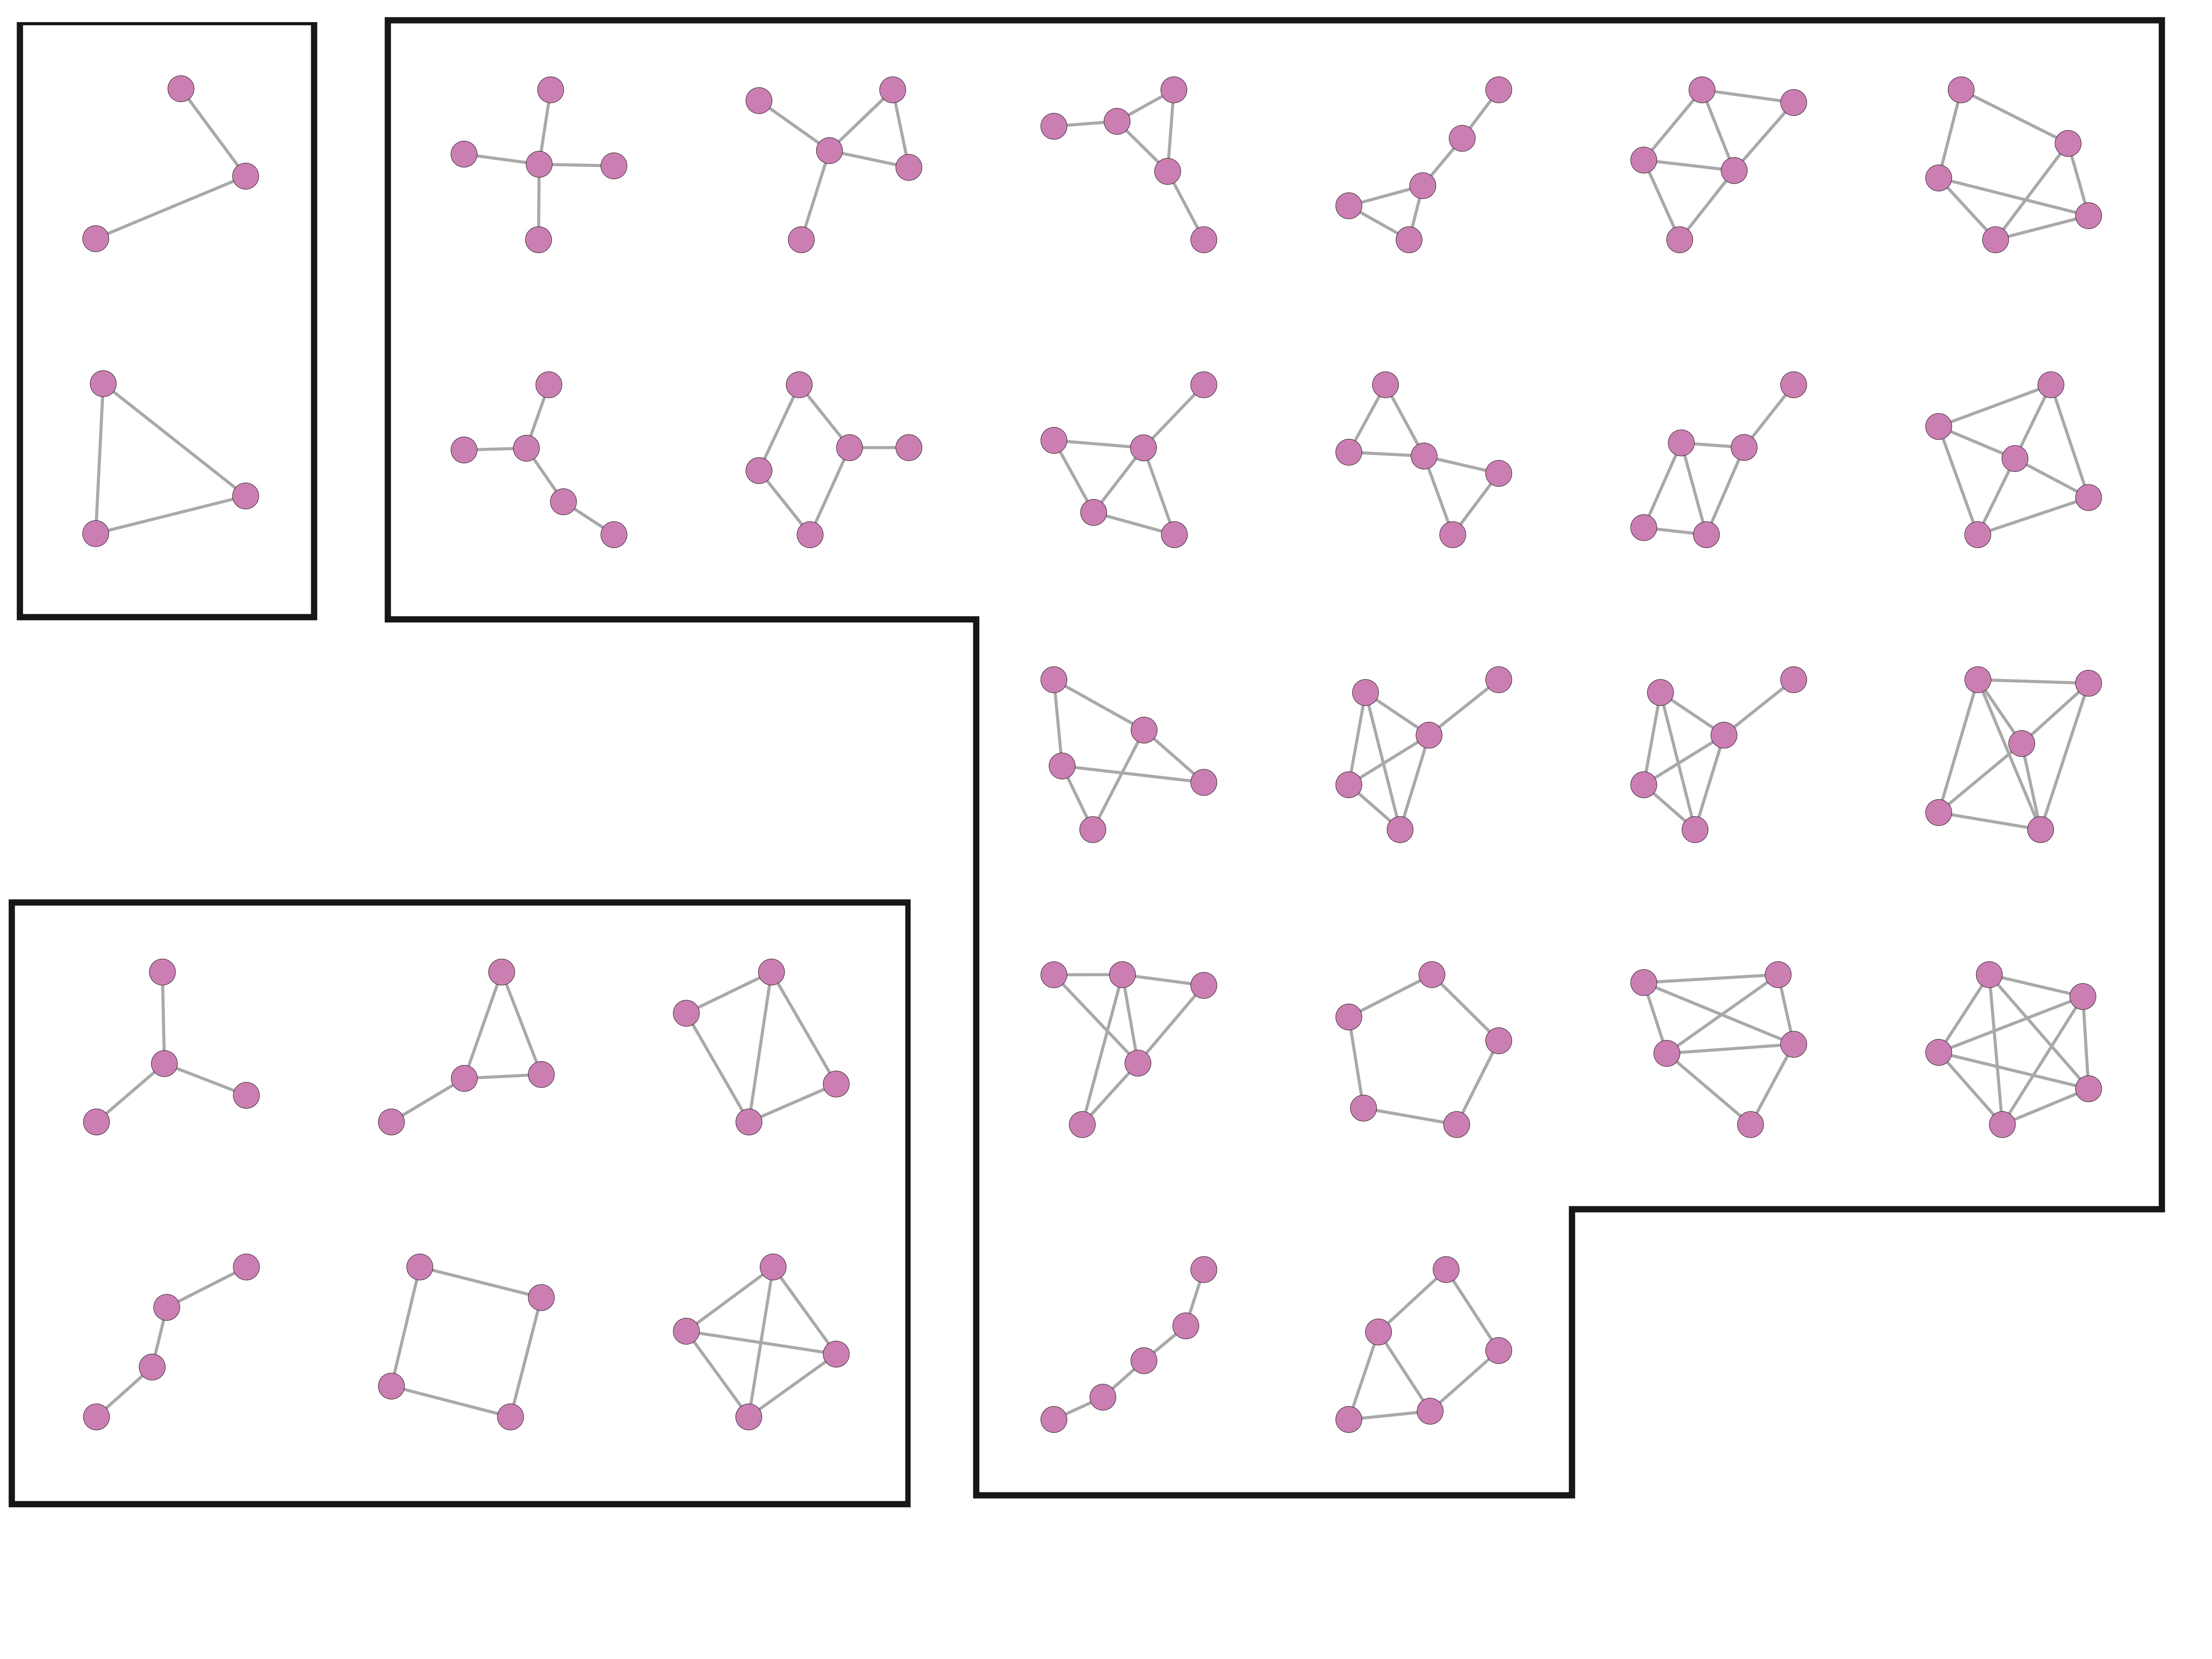
\includegraphics[scale=.07]{figs/subgraphs.png}
\centering
\caption{Potential motifs: sets of order 3, 4, and 5-connected subgraphs}\end{figure}
Network motif discovery essentially follows 3 steps:
\begin{itemize}
\item{Census of subgraphs on original network}
\item{Census of subgraphs on similar random network}
\item{Statistical evaluation of significant motifs}
\end{itemize}
Pedro ribeiro \cite{ribeiro11}, in detailing the short history of network motif discovery algorithms, puts network motif discovery algorithms into two categories: \textit{Network-centric} and \textit{subgraph-centric}. In network-centric approaches, all possible subgraphs of a network are found, afterwards, isomorphism tests are done between graphs to count the frequencies at which each queried subgraph occurs. In subgraph-centric models, a query of the frequency of each subgraph is done on the network. A detailed analysis of different algorithms which use these models is given in \cite{ribeiro11}. Below I will describe the G-Tries algorithm, which, according to analysis done in \cite{ribeiro11} performs an order better than all other algorithms. A comparison of the G-Tries algorithm with the rand-ESU algorithm, which seems to be the next best performing algorithm \cite{li12} is done on the brain networks used in \cite{rubinov10} as well as the neuronal network of the C. elegans, recently revised in \cite{varshney11}. 
\subsection{G-Tries}
The G-Tries algorithm consists of three parts:
\begin{itemize}
\item{Canonical labeling}
\item{Construction of a G-Trie}
\item{Subgraph census}
\end{itemize}
In the G-Tries algorithm, a tree is constructed which is used as a data structure for the subgraph census. Each node of the tree represents a different subgraph, with parent nodes of a current node as connected subgraphs of that current node. As well, the current node is also a connected subgraph of each of its child nodes. The tree, known as a G-Trie (figure 2) for graph-retrieval is constructed using Ribeiro's own canonical labeling algorithm: GTCanon. A canonical labeling is a way of representing a graph such that any graph which is isomorphic to it will have the same canonical labeling. It the GTCanon function, this presents itself as a transfomation on a graphs indexed vertices represented by an array of indexes telling the graph how to swap its vertices in an adjacency matrix to produce the canonical form of that matrix. In the G-Tries algorithm, the canonical labeling also ensures that earlier nodes in a tree have the maximum degree possible while still holding the properties described above. In this way, the G-Trie is constructed in order to have the least possible number of nodes. All of these properties allow the G-Tries algorithm to optimize over its subgraph census.\\
The GTCanon algorithm begins with another canonical labeling algorithm. Ribeiro has chosen \emph{nauty}, which is described in the next section. This pre-canonical labeling is designed to ensure that a graph census can occur on graphs on which GTCanon fails to fulfill the 3 properties described above. So a graph sent into the GTCanon algorithm is converted to canonical form first. After that, a map of the degree of each of it's vertices is made. The algorithm procedes across every position in the previously described transformation array until it is filled, startin from its end, labeling vertex indices which have filled the array thusfar. The algorithm chooses a next label in the following way. The next vertex index in the transformation array must be one which has not yet been added to the array, and the removal of this vertex must not produce a disconnected graph (this ensures that each subgraph in the G-Trie is connected). Out of the remaining candidates to label, the chosen vertex must have the minimum degree with unlabeled vertices out of all of the unlabled vertices. If a vertex index has still not been chosen, the vertex with the minimum degree with all unlabeled vertices plus the last labeled vertex is chosen. If a vertex index is still not chosen, the vertex with the minimum degree with all vertices is chosen. After this, there seems to still be a chance to fail to choose a vertex. Ribeiro suggests to default to making use of the nauty labeling at this point. The author of this paper interprets this as meaning to apply a specific rule at this point which will always ensure a choice, and the choice will always be the same for canonically labeled graphs, such as choosing the vertex with the minimum index. After a new index is chosen to add to the transformation array, the process is repeated until the transformation array is full. The result is an array of indices where the $i$th index tell us where the $i$th vertex will be shifted to in an adjacency matrix.\\
After this, a G-Trie is constructed in the following way. Take the set of subgraphs you want to perform a subgraph census on, apply the GTCanon function to them and iteratively insert them into your G-Trie, which should initially consist of a a root, with no nodes on it. The leaves of this G-Trie should eventually consist of each of the subgraphs you are censusing. The insertion process goes as follows. At each step you add a portion of of a row of the graphs adjacency matrix to the next node, and advance to that node. The portion of the adjacency matrix that you add are the first $k+1$ values of the kth row of your matrix, where $k$ is the depth of the current node. This tells you that the first $k$-indexed vertices of your graph are the same as the child nodes $k$-indexed nodes. If the portion of the adjacency matrix is the same length as the order of the subgraphs you are censusing, you know that you have reached the end of the tree, you add the last portion of the adjacency matrix, and move on to the next subgraph. If not, you look at all of the children of current node, and look at the portion of the adjacency matrix stored there. If it is the same as the $k+1$ values in the $k$th row of the matrix, you advance and store the $k+1$ values in the $k$th row at the new node. Afterwards, a new child is created, at the current node with the $k+1$ values in the $k$th row in the matrix stored on it. The child node becomes the current node, and this process is done recursively until leaf nodes are found for each subgraph. This construction makes a tree which allows for matching of subgraphs in an optimized number of steps.\\ 
The subgraph census is done by taking a node from the graph we are censusing. At each step in the process we add a neighbor to our current subgraph and advance a level in our G-Trie to the node which matches our current subgraph. We know that this exists because each level of the G-Trie corresponds to an order, and contains every kind of connected subgraph for that order at each level. We keep adding neighbors until we get to a leaf node, at which point we know that we have found one of the subgraphs we are censusing, and we add a count to the frequency count for the subgraph. To ensure that the same graph is not found twice the G-Tries algorithm checks for automorphisms using the \emph{nauty} algorithm. This will not be described in the current paper, but as described later, makes up a large part of the time complexity of the algorithm.\\
The current study suggests the use of the GTries algorithm for the speeds that were reported in \cite{ribeiro11} as well as its potential use in an algorithm described in section 6.
\begin{figure}[b!]
\centering
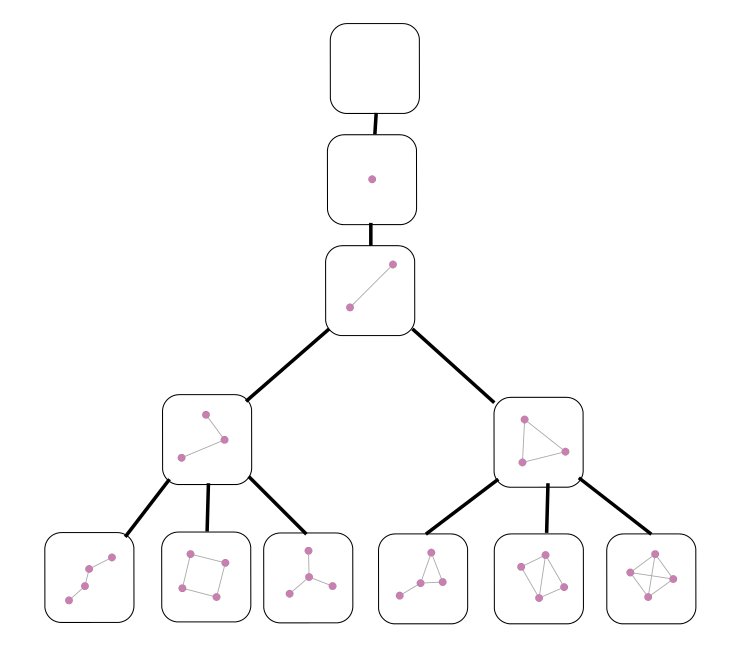
\includegraphics[scale=.25]{figs/gtrie.png}
\caption{A G-Trie containing order 4 connected subgraphs}
\end{figure}

